% TeXplates/Mathematics.tex
% v0.8.0
% https://github.com/HoyanMok/TeXplates
\documentclass[openany, a5paper]{book} 
% \documentclass{ctexbook} 如果用中文
% \documentclass[10pt,a4paper]{ctexart}  字体大小和纸张大小,默认分别为10pt和letterpaper
% 五号 = 10.5pt,小四=12pt,四号=14pt
% 其他可选参量如twocolumn, 两行排版

\usepackage{../TeXplatesMathematics}
\addbibresource{vonNeumannAlgebra.bib} % 把这里改成实际的文件名

% 文章标题页信息:
\title{$C^*$-Algebras}
\author{Hoyan Mok}
\date{\today} % 自动生成日期
\titlepic{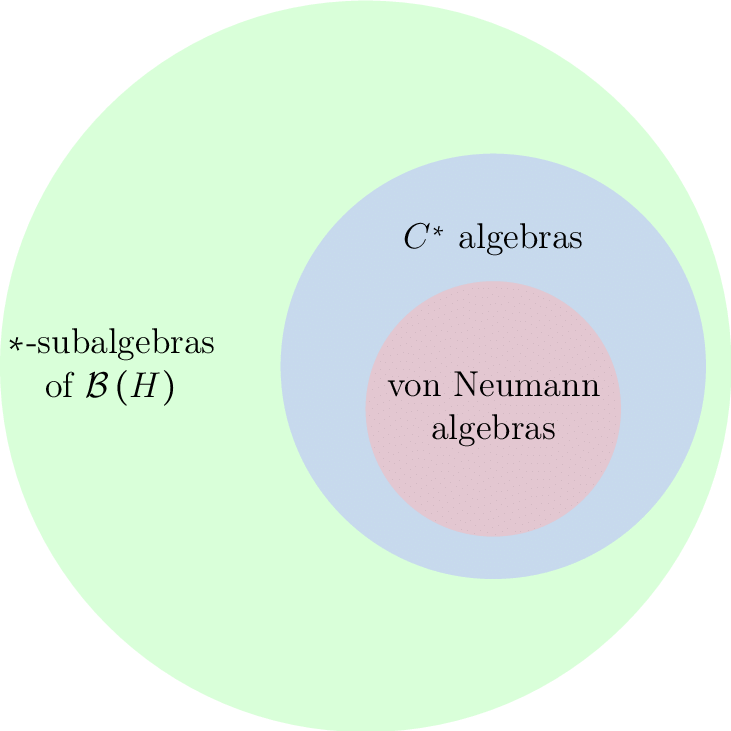
\includegraphics[width=.8\textwidth]{Diagram-to-show-relationship-between-B-H-C-algebras-and-von-Neumann-Algebras.png}}

\begin{document}
\pagenumbering{Alph}
\maketitle % 打印标题
\frontmatter
\chapter{Preface}

$\mathcal H$ means a Hilbert space by default.
If not specified, the base field is $\mathbb K = \mathbb R$ or $\mathbb C$.


\tableofcontents

\mainmatter
\chapter{Banach Algebras}
\section{Banach Algebras \& Invertible Group}

\begin{definition}[Banach algebra]
    A \indexbf{Banach algebra} is a unital algebra $\mathscr B$ together with a norm $\|\dummy\|$ s.t.\
    \begin{enumerate}
        \item $\|1_{\mathscr B}\| = 1$;
        \item $\forall a, b \in \mathscr B,\; \|ab\| \leq \|a\| \|b\|$.
    \end{enumerate}
\end{definition}

The most important example of Banach algebras may be the algebra $B(\mathcal H)$ of bounded linear operators on a Banach space $\mathcal H$ with the operator norm:
\begin{equation}
    \|L\|_{B(\mathcal H)} = \sup_{\|v\| = 1} \|Lv\|.
\end{equation}


\chapter{\texorpdfstring{$C^*$-Algebras}{C*-Algebras}}
\section{\texorpdfstring{$C^*$-Algebras}{C*-Algebras}}

\begin{definition}[$C^*$-algebra]
    A \indexbf{$C^*$-algebra} is a Banach algebra $\mathscr A$ together with an \indexbf{involution} $* \colon \mathscr A \to \mathscr A$ s.t.\ 
    \begin{enumerate}
        \item $\forall a \in \mathscr A$, $a^{**} = a$;
        \item $\forall a, b \in \mathscr A$, $(ab)^* = b^* a^*$;
        \item $\forall a, b \in \mathscr A$, $\forall \alpha, \beta \in \mathbb K$,
            $(\alpha a + \beta b)^* = \overline \alpha a^* + \overline \beta b^*$\footnote{%
                If $\mathbb K = \mathbb R$, then $\overline \alpha := \alpha$.
            };
        \item $\forall a \in \mathscr A$, $\|a^* a\| = \|a\|^2$.
    \end{enumerate}

    The element $a^*$ is called the \indexbf{adjoint} of $a$.
\end{definition}

\begin{definition}[Projection]
    An element $p \in \mathscr A$ is called a \indexbf{projection} if $p^2 = p = p^*$.
\end{definition}

\section{\texorpdfstring{Commutative $C^*$-Algebras}{Commutative C*-Algebras}}

\appendix
\renewcommand{\theequation}{\Alph{chapter}-\arabic{equation}}
\chapter{Appendix}

\backmatter
\nocite{*} % 这个表示列出所有没有在文中被引用的参考文献
\printbibliography[heading=bibliography, title={Bibliography}]

\indexprologue{Here listed the important symbols used in this notes.}
\printindex[symbol]

\printindex

\end{document}